\documentclass[type=dr, dr=rernat, accentcolor=tud7b,colorbacktitle, bigchapter, openright, twoside, 12pt ]{tudthesis}
%\documentclass[11pt,twoside,a4paper]{article}
\usepackage[english]{babel} 
\usepackage[utf8]{inputenc}
\usepackage{graphicx}
\usepackage{pstricks}
\usepackage{psfrag}
\usepackage{enumerate}
\usepackage{float}
\usepackage{epsfig}
\usepackage{geometry}
\usepackage{subfigure}
\usepackage{rotating}
\usepackage{minitoc}
%\usepackage{appendix}

%%%% 1 1/2 facher Zeilenabstand:	
\usepackage{setspace}
\onehalfspacing




\begin{document}
\chapter{Research background and Fundamentals}
\label{chapter:intro}
\minitoc

\section{Radiotherapy}

Since the discovery of X-rays in 1895 the radiation has been used by physicans for treating patients. 
In the begining only superfical diseases could be cured, but as time and technology progressed X-ray tubes gained on voltage
and allowing treatment of deeper suited tumors.

The radiation from linear accelerator was first used in medicine in 1953. Because the beam is more collimated and energies are
higher than X-ray tube the cure rates improved tremendously. The next big milestone was introduction of computeres in the field
of radiotherapy. This led to better diagnostic tools, such as computed tomography scans (CT), magnetic resonance imaging (MRI) and
positron emission tomography (PET). With those tools the location of the tumor could be much better estimated and hence the physicans
could easier prescribe treatment. The potential of computers were afterwards exploited also in treatment planning with intensity modulated
radiation therapy (IMRT) which, together with diagnostic tools, provides an exact dose shaping in accordance to patient specific tumors.

In 1946 it was discovered that protons could be used alongside photons for cancer treatment. Furthermore it was shown that protons have preferable depth dose profile 
compared to photons. First patient treatment soon followed in the early 1950's at Lawrence Berkeley Laboratory, USA. Heavier ions, such as 
He$^{2+}$, $^{20}$Ne and $^6$C were also used later on for treatment. In the begining only passive beam delivery was used for treatment 
and in the 1990's active beam solutions were developed at Paul Scherrer Institut (PSI), Villigen (Switzerland) for protons and at GSI, Darmstadt 
(Germany) for carbon ions.

Both treatment modalities (photons and ions) use the same principle to eliminate cancer cells. The physical and biological mechanism behind 
it will be explained in detail in the following sections.


\section{Physcial and biological basics of radiotherapy}

\subsection{Interaction of radiation with matter}

The interactions between photons and ions with matter are quite different. Photons deposit highest local dose shortly after entering the matter (at the energies used in radiotherapy).
Ions 

\newpage
 
\vspace*{1cm}
 
\begin{figure}[H]
\begin{center}
% 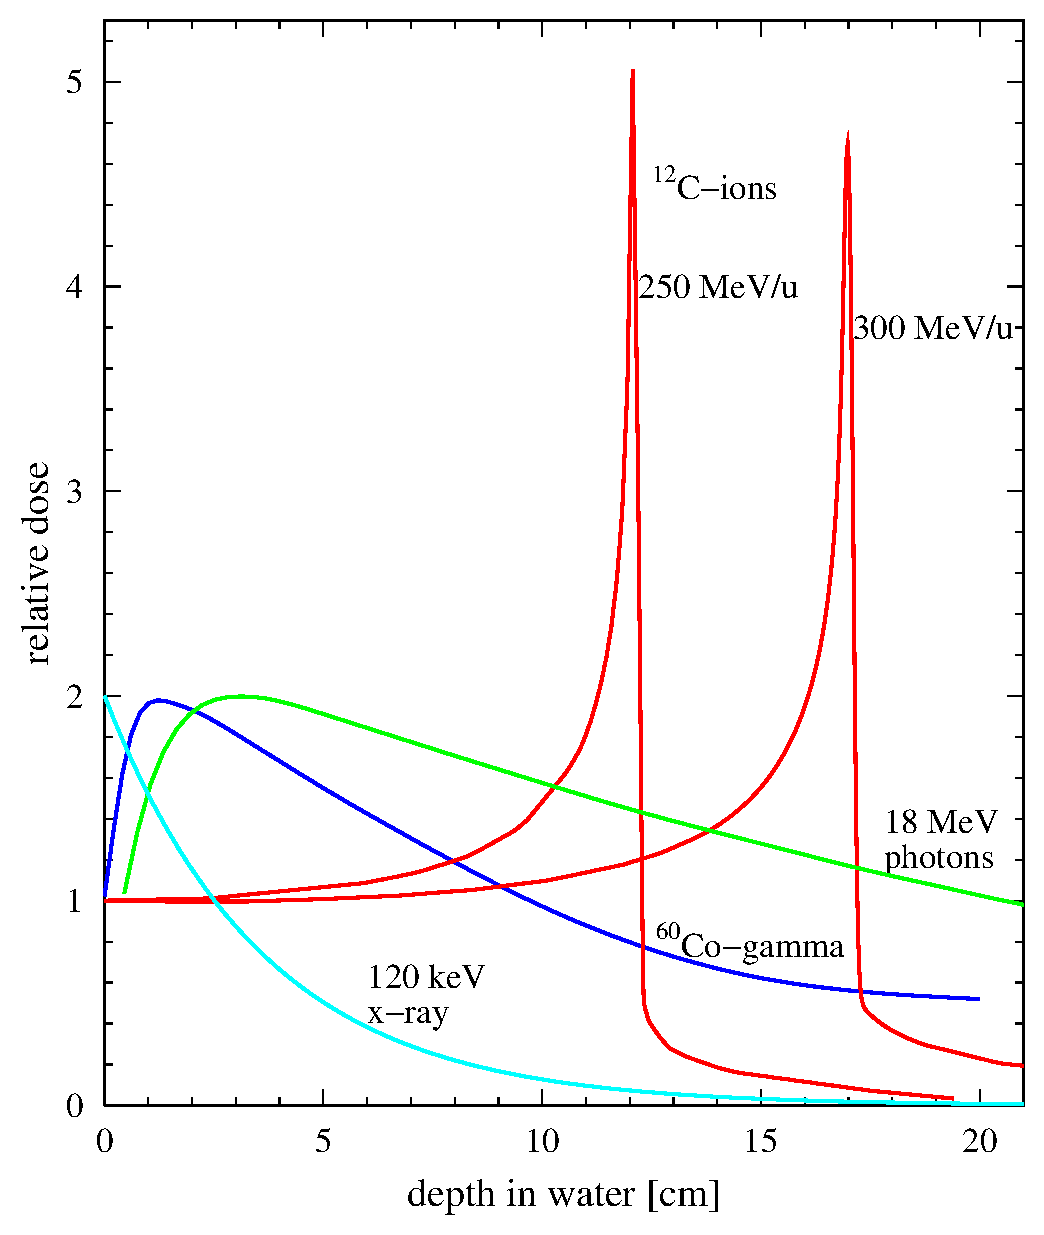
\includegraphics[scale=1]{depthdose.eps}
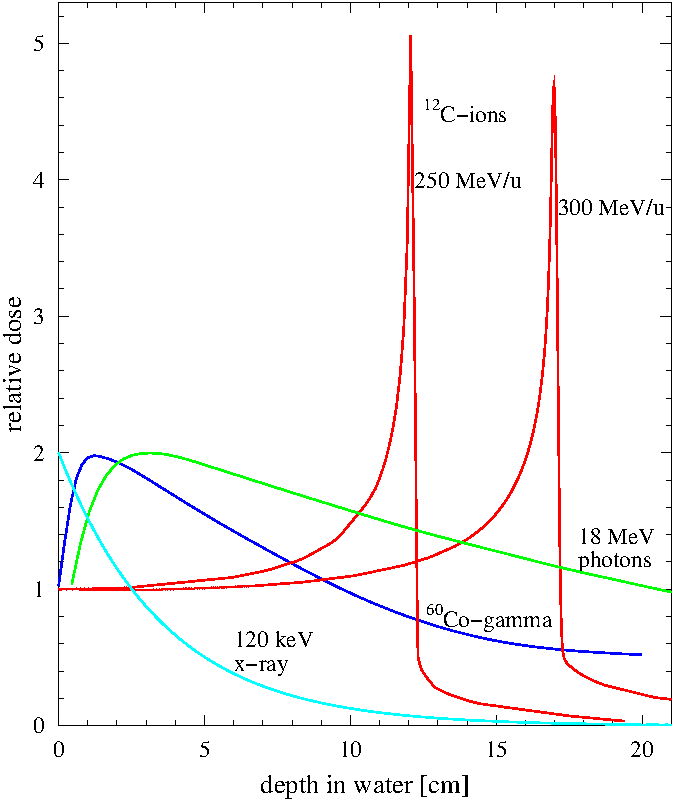
\includegraphics[scale=1]{depthdose.png}
\caption{Depth dose distributions of photons and carbon ions at different energies. Photons display an exponential decrease after a certain 
build up. Ions on the other hand interact differently with matter, resulting in an increased dose deposition at the end of the particle 
track, the Bragg peak. Figure taken from \cite{Schardt2010} }
\label{ddp}
\end{center}
\end{figure}
% 
% *\include{ref.bib}
\bibliographystyle{apalike}
\bibliography{ref}
% \bibliographystyle{plain}

\end{document}